\documentclass[11pt,a4paper]{report}

% =============================================================================
% PREAMBLE & PACKAGES
% =============================================================================
\usepackage{iftex}
\ifPDFTeX
  \usepackage[T1]{fontenc}
  \usepackage[utf8]{inputenc}
  \usepackage[english]{babel}
  \usepackage{lmodern}
\else
  \usepackage{fontspec}
  \setmainfont{Liberation Serif}
  \setsansfont{Liberation Sans}
  \setmonofont{Liberation Mono}
  \usepackage[english]{babel}
\fi

\usepackage[top=2.5cm,bottom=2.5cm,left=3cm,right=2cm]{geometry}
\usepackage{amsmath,amssymb,amsfonts,mathtools}
\usepackage{graphicx}
\usepackage{tikz}
\usetikzlibrary{positioning,shapes.geometric,arrows.meta,shadows,trees,calc,backgrounds}
\usepackage{booktabs}
\usepackage{multirow}
\usepackage{tabularx}
\usepackage{array}
\usepackage{listings}
\usepackage{xcolor}
\usepackage{hyperref}
\usepackage{url}
\usepackage{cite}
\usepackage{fancyhdr}
\usepackage{titlesec}
\usepackage{enumitem}

% Color Definitions
\definecolor{navyblue}{RGB}{0,32,96}
\definecolor{darkgreen}{RGB}{0,100,0}
\definecolor{codegray}{rgb}{0.5,0.5,0.5}
\definecolor{backcolour}{rgb}{0.96,0.96,0.96}
\definecolor{cypherblue}{RGB}{28,112,184}
\definecolor{codepurple}{rgb}{0.58,0,0.82}

% Code Listing Configuration
\lstdefinestyle{codeStyle}{
    backgroundcolor=\color{backcolour},
    commentstyle=\color{darkgreen},
    keywordstyle=\color{navyblue}\bfseries,
    numberstyle=\tiny\color{codegray},
    stringstyle=\color{red!70!black},
    basicstyle=\ttfamily\footnotesize,
    breakatwhitespace=false,
    breaklines=true,
    captionpos=b,
    keepspaces=true,
    numbers=left,
    numbersep=5pt,
    showspaces=false,
    showstringspaces=false,
    showtabs=false,
    tabsize=2
}
\lstset{style=codeStyle}

% Hyperlink setup
\hypersetup{
    unicode=true,
    colorlinks=true,
    linkcolor=navyblue,
    citecolor=darkgreen,
    urlcolor=blue,
    pdftitle={Course Report Knowledge Representation - HLG LLM Utils Graph RAG},
    pdfauthor={Nguyen Hoai Nam, Pham Cung Le Nhan Vu}
}

% Header and Footer
\pagestyle{fancy}
\fancyhf{}
\setlength{\headheight}{14pt}
\rhead{\small\itshape Graph RAG}
\lhead{\small\itshape Knowledge Representation -- Assoc. Prof. Dr. Do Van Nhon}
\cfoot{\thepage}

% Section Title Formatting
\titleformat{\chapter}[display]
  {\normalfont\bfseries\color{navyblue}\Large}
  {\chaptertitlename\ \thechapter}{10pt}{\Huge}
\titleformat{\section}
  {\normalfont\bfseries\color{navyblue}\Large}
  {\thesection}{1em}{}
\titleformat{\subsection}
  {\normalfont\bfseries\color{navyblue}\large}
  {\thesubsection}{1em}{}
\titleformat{\subsubsection}
  {\normalfont\bfseries\color{navyblue}\normalsize}
  {\thesubsubsection}{1em}{}

% =============================================================================
% DOCUMENT BEGINS
% =============================================================================
\begin{document}

% -----------------------------------------------------------------------------
% TITLE PAGE
% -----------------------------------------------------------------------------
\begin{titlepage}
    \centering
    \vspace*{0.5cm}
    {\Large\bfseries VIETNAM NATIONAL UNIVERSITY HO CHI MINH CITY}\\[0.2cm]
    {\large\bfseries UNIVERSITY OF SCIENCE -- FACULTY OF INFORMATION TECHNOLOGY}\\[0.1cm]
    {\large\bfseries DEPARTMENT OF COMPUTER SCIENCE}\\[1.5cm]

    {\Large\bfseries COURSE RESEARCH REPORT}\\[0.3cm]
    {\Huge\bfseries\color{navyblue} KNOWLEDGE REPRESENTATION}\\[0.8cm]

    \begin{center}
    \fbox{
    \begin{minipage}{0.92\textwidth}
    \centering
    \vspace{0.3cm}
    {\Large\bfseries\color{navyblue} Topic: HLG LLM UTILS -- AN ADVANCED GRAPH RAG FRAMEWORK WITH MULTI-AGENT ORCHESTRATION, HIERARCHICAL LEIDEN COMMUNITY DETECTION, AND CYPHER QUERY SELF-CORRECTION}\\[0.2cm]
    \vspace{0.3cm}
    \end{minipage}
    }
    \end{center}

    \vspace{1.2cm}

    \begin{minipage}{0.85\textwidth}
        \large
        \begin{tabular}{ll}
            \textbf{Instructor:} & Assoc. Prof. Dr. Do Van Nhon \\[0.3cm]
            \textbf{Students:} & 1. Nguyen Hoai Nam -- Student ID: 25C01014 \\[0.15cm]
            & 2. Pham Cung Le Nhan Vu -- Student ID: 25C01049 \\[0.3cm]
            \textbf{Major:} & Data Science \\[0.15cm]
            \textbf{Intake:} & K35
        \end{tabular}
    \end{minipage}

    \vfill
    {\large Ho Chi Minh City -- Year 2026}
\end{titlepage}

% -----------------------------------------------------------------------------
% ABSTRACT & FRONTMATTER
% -----------------------------------------------------------------------------
\pagenumbering{roman}
\setcounter{page}{1}

\section*{Executive Abstract}
\addcontentsline{toc}{chapter}{Executive Abstract}

Standard Retrieval-Augmented Generation (\textbf{Naive RAG}) systems based on flat text chunking and vector space similarity (e.g., \textbf{Cosine Similarity} over high-dimensional embeddings) face two fundamental bottlenecks in Knowledge Representation and Information Retrieval: (1) Inability to address corpus-wide macro-summarization queries (\textbf{Global Queries}) due to structural context fragmentation; and (2) Failure in multi-hop reasoning (\textbf{Multi-Hop Reasoning}) across complex relational entity dependency chains.

This report comprehensively presents the design, mathematical formalization, and engineering implementation of \textbf{HLG LLM Utils}, a production-grade \textbf{Graph RAG} framework built upon a decoupled Python monorepo architecture (\texttt{uv workspaces}). The system tightly integrates Neo4j Property Knowledge Graphs with Large Language Models, delivering four core retrieval and reasoning engines:
\begin{enumerate}[leftmargin=*]
    \item \textbf{Property Knowledge Graph Formalization:} Formal mathematical modeling and automated extraction of entities, relationships, attributes, and source document lineages from unstructured text into Neo4j using idempotent \texttt{MERGE} operations.
    \item \textbf{Hierarchical Leiden Community Detection:} Implementing modularity optimization over \texttt{igraph} and \texttt{leidenalg} to construct multi-level community hierarchies, accompanied by parallel LLM summarization for Map-Reduce global search.
    \item \textbf{LangGraph Cypher Query Self-Correction State Machine:} A deterministic state graph translating natural language into executable Cypher queries with an automated 3-iteration error feedback loop against Neo4j execution logs.
    \item \textbf{ARK (Adaptive Retriever of Knowledge) Multi-Agent Exploration:} Implementing stochastic multi-agent trajectory exploration (ACL 2026) with Voting Rank Fusion (VRF) to adaptively balance search breadth and depth across the graph.
\end{enumerate}

This report covers the theoretical foundations, database schema designs, software architecture, and algorithm implementations actually deployed in the codebase.

\textbf{Keywords:} Graph RAG, Knowledge Representation, Property Knowledge Graph, Hierarchical Leiden Algorithm, Cypher Self-Correction, Multi-Agent Systems, LangGraph, Adaptive Retriever of Knowledge, Monorepo uv.

\newpage
\tableofcontents
\newpage
\listoffigures
\listoftables
\newpage

% -----------------------------------------------------------------------------
% MAIN CONTENT CHAPTERS
% -----------------------------------------------------------------------------
\pagenumbering{arabic}
\setcounter{page}{1}

% =============================================================================
\chapter{Introduction \& Problem Statement}
% =============================================================================

\section{Background \& Motivation}
In modern artificial intelligence, Large Language Models (\textbf{LLMs}) have demonstrated extraordinary capabilities in natural language understanding and generation. Nevertheless, purely parametric models suffer from two intrinsic limitations: the risk of generating ungrounded or fabricated information (\textbf{Hallucination}) and knowledge staleness due to static parameter weights. To mitigate these shortcomings, \textbf{Retrieval-Augmented Generation (RAG)} has emerged as the standard paradigm for grounding LLMs with external knowledge repositories \cite{lewis2020rag}.

However, first-generation RAG systems (\textbf{Naive RAG}) -- which rely on cutting documents into fixed-size text chunks and retrieving them through vector embedding similarity -- exhibit severe limitations when handling complex Knowledge Representation tasks.

\section{Core Bottlenecks of Naive Flat RAG}
Through theoretical analysis and practical implementation, we identify three critical bottlenecks of flat vector RAG:

\begin{enumerate}[leftmargin=*]
    \item \textbf{Structural Context Fragmentation:} Splitting text into fixed chunks $c_i \in \mathcal{C}$ (e.g., 500 or 1000 tokens) arbitrarily destroys relational semantics spanning across multiple paragraphs or documents. When entity $E_1$ defined in chunk $c_1$ shares a causal relationship with entity $E_2$ in chunk $c_k$, this semantic connection is lost in flat vector space.
    \item \textbf{Multi-Hop Reasoning Failures:} Consider a multi-hop query requiring transitive inference:
    \begin{equation}
        E_{\text{start}} \xrightarrow{R_1} E_{\text{mid}} \xrightarrow{R_2} E_{\text{target}}
    \end{equation}
    When a user query asks about $E_{\text{start}}$ and $E_{\text{target}}$, standard \textbf{Cosine Similarity} retrieval only surfaces chunks directly mentioning $E_{\text{start}}$ or $E_{\text{target}}$, completely omitting the intermediate bridge entity $E_{\text{mid}}$. The resulting context is insufficient for LLM reasoning.
    \item \textbf{Global Query Blindspots:} For macro-level summarization queries (e.g., \textit{"What are the main thematic clusters discussed in this dataset?"} or \textit{"Summarize organizational interactions"}), the query vector $\mathbf{q} \in \mathbb{R}^d$ exhibits low similarity with any single chunk, rendering Naive RAG entirely ineffective \cite{edge2024graphrag}.
\end{enumerate}

\section{Research Objectives \& Core Contributions}
To address these challenges, this project investigates, designs, and implements \textbf{HLG LLM Utils} -- a comprehensive \textbf{Graph RAG} framework combining Neo4j Property Knowledge Graphs with advanced multi-agent and community detection algorithms.

Key contributions include:
\begin{itemize}[leftmargin=*]
    \item \textbf{Mathematical Modeling \& Schema Architecture:} Formalizing the Property Knowledge Graph $G = (\mathcal{V}, \mathcal{E}, \mathcal{P}, \mathcal{W})$, designing storage schemas for \texttt{:Entity}, \texttt{:Chunk}, \texttt{:Document}, and \texttt{:Community} nodes alongside their respective relationship types.
    \item \textbf{Idempotent Graph Ingestion Pipeline:} Implementing structured entity/relationship extraction using Pydantic schemas and LLM invocation, stored asynchronously into Neo4j via idempotent \texttt{MERGE} statements.
    \item \textbf{Hierarchical Leiden Community Detection:} Implementing multi-level modularity optimization with \texttt{igraph} and \texttt{leidenalg}, generating hierarchical community trees and parallel LLM summaries for Map-Reduce global search.
    \item \textbf{LangGraph Cypher Self-Correction State Machine:} Building a deterministic state graph for natural-language-to-Cypher translation with a 3-iteration feedback loop driven by Neo4j execution logs.
    \item \textbf{ARK Multi-Agent Exploration:} Implementing the Adaptive Retriever of Knowledge algorithm with Voting Rank Fusion (VRF) to dynamically balance graph traversal breadth and depth.
    \item \textbf{Modular Monorepo Architecture:} Packaging the system into a clean \texttt{uv workspaces} monorepo, integrating FastAPI backend services and FastMCP standard tooling.
\end{itemize}

% =============================================================================
\chapter{Theoretical Foundations \& Related Work}
% =============================================================================

\section{From Semantic Networks to Property Knowledge Graphs}
Knowledge Representation (\textbf{KR}) is a foundational pillar of Artificial Intelligence, formalizing real-world domain knowledge into computable structures for automated reasoning \cite{ji2022survey}.

\subsection{Semantic Networks and RDF Triples}
Traditional semantic networks represent knowledge as nodes (concepts) and directed edges (relations). In the W3C Semantic Web stack, knowledge is formalized into RDF triples (\textit{Subject, Predicate, Object}):
\begin{equation}
    \tau = (s, p, o) \in \mathcal{E} \times \mathcal{R} \times (\mathcal{E} \cup \mathcal{L})
\end{equation}
While standardized, RDF lacks native support for attaching rich auxiliary properties (metadata, confidence scores, source citations, timestamps) directly onto relationships.

\subsection{Labeled Property Graph (LPG) Model}
The \textbf{Labeled Property Graph (LPG)} model solves this limitation by allowing both vertices (nodes) and edges (relationships) to maintain type labels and arbitrary sets of key-value property maps \cite{robinson2015graph}:
\begin{equation}
    G = (\mathcal{V}, \mathcal{E}, \lambda_V, \lambda_E, \rho_V, \rho_E)
\end{equation}
The LPG model enables direct representation of entity descriptions, taxonomy types, vector embeddings, and source document provenance on graph elements.

\section{Vector Space Embeddings \& Hybrid Retrieval}
In continuous vector spaces, each text segment or entity $x$ is mapped to a high-dimensional feature vector $\mathbf{e}_x \in \mathbb{R}^d$ via Transformer encoders \cite{reimers2019sentencebert}:
\begin{equation}
    \mathbf{e}_x = \text{Embed}(x) \in \mathbb{R}^d, \quad \|\mathbf{e}_x\|_2 = 1
\end{equation}
The semantic similarity between query $q$ and entity $x$ is given by Cosine Similarity:
\begin{equation}
    \text{Sim}(q, x) = \langle \mathbf{e}_q, \mathbf{e}_x \rangle = \sum_{i=1}^d e_{q,i} \cdot e_{x,i}
\end{equation}

Our system combines keyword search (\textbf{BM25 / Fulltext Index}) and dense vector search (\textbf{Dense Vector Index}) via \textbf{Reciprocal Rank Fusion (RRF)} \cite{cormack2009rrf}:
\begin{equation}
    \text{RRF\_Score}(d) = \sum_{m \in \{\text{Vector}, \text{Fulltext}\}} \frac{1}{k_{\text{rrf}} + \text{rank}_m(d)}
\end{equation}
with smoothing constant $k_{\text{rrf}} = 60$.

\section{Graph Partitioning \& The Leiden Algorithm}
Graph partitioning divides the vertex set $\mathcal{V}$ into disjoint communities $\mathcal{P} = \{C_1, C_2, \dots, C_k\}$ such that internal edge density is maximized while inter-community edges are minimized \cite{traag2019leiden}.

\subsection{Modularity Optimization}
The modularity $Q$ of a partition on an undirected graph $G = (\mathcal{V}, \mathcal{E})$ with total weight $m = \frac{1}{2}\sum_{ij} A_{ij}$ is defined as:
\begin{equation}
    Q = \frac{1}{2m} \sum_{i,j \in \mathcal{V}} \left[ A_{ij} - \gamma \frac{k_i k_j}{2m} \right] \delta(C(i), C(j))
\end{equation}
where $A_{ij}$ is the adjacency matrix, $k_i$ is node degree, $\gamma$ is the resolution parameter, and $\delta$ is the Kronecker delta function.

\subsection{The Leiden Guarantee Over Louvain}
The classical Louvain algorithm frequently produces disconnected communities. The \textbf{Leiden} algorithm \cite{traag2019leiden} guarantees well-connected communities through a three-phase cycle:
\begin{enumerate}
    \item \textbf{Local Movement of Nodes:} Moving individual nodes to neighboring communities to maximize quality.
    \item \textbf{Refinement of Partition:} Sub-clustering communities to guarantee internal connectivity.
    \item \textbf{Aggregation of Graph:} Contracting the graph based on refined partitions and repeating recursively.
\end{enumerate}

\section{Adaptive Multi-Agent Knowledge Retrieval (ARK)}
The \textbf{ARK} framework \cite{polonuer2026ark} (ACL 2026) models knowledge retrieval as a distributed search problem across multiple stochastic agents. Agents dynamically choose actions at each step -- global search, local neighborhood expansion, or selecting answer candidates -- adapting traversal depth and breadth based on query complexity.

% =============================================================================
\chapter{Formal Knowledge Representation \& Schema Design}
% =============================================================================

\section{Mathematical Property Knowledge Graph Model}
The knowledge graph in HLG LLM Utils is formalized as:
\begin{equation}
    \mathcal{G} = (\mathcal{V}, \mathcal{E}, \mathcal{P}_V, \mathcal{P}_E, \ell_V, \ell_E)
\end{equation}
where:
\begin{itemize}[leftmargin=*]
    \item $\mathcal{V} = \mathcal{V}_{\text{Entity}} \cup \mathcal{V}_{\text{Chunk}} \cup \mathcal{V}_{\text{Doc}} \cup \mathcal{V}_{\text{Comm}}$ partitions vertices into entities, text chunks, documents, and communities.
    \item $\mathcal{E} \subseteq \mathcal{V} \times \mathcal{V}$ denotes the set of directed edges.
    \item $\ell_V: \mathcal{V} \to \{\text{Entity}, \text{Chunk}, \text{Document}, \text{Community}\}$ assigns vertex labels.
    \item $\ell_E: \mathcal{E} \to \{\text{RELATED\_TO}, \text{BELONGS\_TO}, \text{CONTAINS\_CHUNK}, \text{MENTIONS}, \text{PARENT\_COMMUNITY}\}$ assigns relationship types.
    \item $\mathcal{P}_V(v)$ and $\mathcal{P}_E(e)$ define property attribute maps.
\end{itemize}

\section{Neo4j Graph Database Schema Architecture}
The graph schema is optimized for both relational graph traversals and semantic vector indexing:

\begin{figure}[h!]
\centering
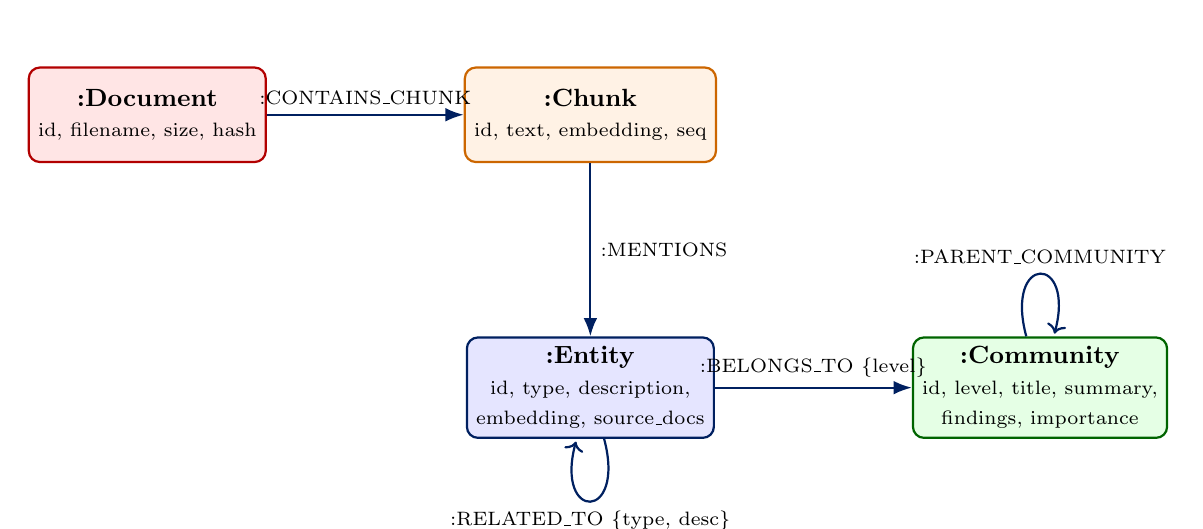
\begin{tikzpicture}[
    node distance=2.2cm and 2.5cm,
    every node/.style={font=\small},
    entityNode/.style={rectangle, draw=navyblue, fill=blue!10, thick, rounded corners, minimum height=1.2cm, minimum width=2.8cm, align=center},
    commNode/.style={rectangle, draw=darkgreen, fill=green!10, thick, rounded corners, minimum height=1.2cm, minimum width=2.8cm, align=center},
    docNode/.style={rectangle, draw=red!70!black, fill=red!10, thick, rounded corners, minimum height=1.2cm, minimum width=2.8cm, align=center},
    chunkNode/.style={rectangle, draw=orange!80!black, fill=orange!10, thick, rounded corners, minimum height=1.2cm, minimum width=2.8cm, align=center},
    relEdge/.style={draw=navyblue, -Latex, thick}
]
    \node [docNode] (doc) {\textbf{:Document}\\\scriptsize id, filename, size, hash};
    \node [chunkNode, right=of doc] (chunk) {\textbf{:Chunk}\\\scriptsize id, text, embedding, seq};
    \node [entityNode, below=of chunk] (entity) {\textbf{:Entity}\\\scriptsize id, type, description,\\\scriptsize embedding, source\_docs};
    \node [commNode, right=of entity] (comm) {\textbf{:Community}\\\scriptsize id, level, title, summary,\\\scriptsize findings, importance};

    \path [relEdge] (doc) -- node[above]{\scriptsize :CONTAINS\_CHUNK} (chunk);
    \path [relEdge] (chunk) -- node[right]{\scriptsize :MENTIONS} (entity);
    \path [relEdge] (entity) edge [loop below] node[below]{\scriptsize :RELATED\_TO \{type, desc\}} (entity);
    \path [relEdge] (entity) -- node[above]{\scriptsize :BELONGS\_TO \{level\}} (comm);
    \path [relEdge] (comm) edge [loop above] node[above]{\scriptsize :PARENT\_COMMUNITY} (comm);
\end{tikzpicture}
\caption{Neo4j Property Knowledge Graph Schema Architecture}
\label{fig:neo4j_schema_en}
\end{figure}

\subsection{Node Attributes Specification}
\begin{enumerate}[leftmargin=*]
    \item \textbf{Entity Node (\texttt{:Entity}):}
    \begin{itemize}
        \item \texttt{id}: Primary key (normalized uppercase string, e.g., \texttt{"GRAPH RAG"}).
        \item \texttt{type}: Semantic classification (e.g., \texttt{"CONCEPT"}, \texttt{"ALGORITHM"}, \texttt{"FRAMEWORK"}).
        \item \texttt{description}: Detailed textual definition of the entity.
        \item \texttt{embedding}: High-dimensional semantic vector $\mathbf{e} \in \mathbb{R}^d$ ($d=1536$ or $d=768$).
        \item \texttt{source\_documents}: Array of source document filenames containing this entity.
    \end{itemize}
    \item \textbf{Community Node (\texttt{:Community}):}
    \begin{itemize}
        \item \texttt{id}: Unique level-scoped identifier (e.g., \texttt{"community\_lvl0\_14"}).
        \item \texttt{level}: Tree hierarchy level ($l \in \{0, 1, \dots, L_{\text{max}}-1\}$).
        \item \texttt{title}: Concise descriptive summary title ($\le 10$ words).
        \item \texttt{summary}: Synthesized thematic summary generated by LLM.
        \item \texttt{findings}: Key analytical findings and insights.
        \item \texttt{importance\_score}: Importance weight metric ($s \in [0.0, 1.0]$).
        \item \texttt{entity\_count}: Number of member entities belonging to the community.
    \end{itemize}
\end{enumerate}

\section{Specialized Indices Configuration on Neo4j}
To optimize multi-modal search, the system initializes specialized vector and fulltext indices:
\begin{itemize}[leftmargin=*]
    \item \textbf{Vector Index on Entity (\texttt{entity\_embeddings}):}
    \begin{lstlisting}[language=SQL,basicstyle=\ttfamily\scriptsize]
CREATE VECTOR INDEX `entity_embeddings` IF NOT EXISTS
FOR (n:Entity) ON (n.embedding)
OPTIONS {indexConfig: {
  `vector.dimensions`: $dimension,
  `vector.similarity_function`: 'cosine'
}}
    \end{lstlisting}
    \item \textbf{Vector Index on Community (\texttt{community\_embeddings}):}
    \begin{lstlisting}[language=SQL,basicstyle=\ttfamily\scriptsize]
CREATE VECTOR INDEX `community_embeddings` IF NOT EXISTS
FOR (c:Community) ON (c.embedding)
OPTIONS {indexConfig: {
  `vector.dimensions`: $dimension,
  `vector.similarity_function`: 'cosine'
}}
    \end{lstlisting}
    \item \textbf{Fulltext Index on Entity (\texttt{entity\_fulltext}):}
    \begin{lstlisting}[language=SQL,basicstyle=\ttfamily\scriptsize]
CREATE FULLTEXT INDEX entity_fulltext IF NOT EXISTS
FOR (n:Entity) ON EACH [n.id, n.description, n.type]
    \end{lstlisting}
\end{itemize}

% =============================================================================
\chapter{Graph Indexing \& Ingestion Pipeline}
% =============================================================================

\section{Preprocessing \& Chunking Pipeline}
The document ingestion pipeline is orchestrated by \texttt{DocumentService}:
\begin{enumerate}
    \item Raw files (PDF, Docx, Code) are retrieved from MinIO S3 storage and converted to plain text via \texttt{llm-utils-parser} (using PyMuPDF for PDFs and OCR engines where needed).
    \item Text is split via sliding token windows ($W = 1000$ tokens, overlap $O = 200$ tokens).
    \item Text chunks are indexed into PostgreSQL and vector stores (Qdrant / PGVector).
\end{enumerate}

\section{Structured Extraction with Pydantic Models}
Structured entity and relationship extraction is enforced via Pydantic models in \texttt{indexing.py}:

\begin{lstlisting}[language=Python,basicstyle=\ttfamily\scriptsize]
class EntityModel(BaseModel):
    id: str
    type: str = "CONCEPT"
    description: str = ""

class RelationshipModel(BaseModel):
    source: str
    target: str
    type: str = "RELATED_TO"
    description: str = ""

class ExtractionResult(BaseModel):
    entities: List[EntityModel] = Field(default_factory=list)
    relationships: List[RelationshipModel] = Field(default_factory=list)
\end{lstlisting}

\section{Idempotent Cypher MERGE Ingestion}
To ensure deterministic, duplicate-free graph ingestion across multiple runs, \texttt{indexing.py} executes idempotent \texttt{MERGE} operations:

\begin{lstlisting}[language=SQL,basicstyle=\ttfamily\scriptsize]
MERGE (e:Entity {id: $id})
ON CREATE SET e.type = $type,
              e.description = $description,
              e.embedding = $embedding,
              e.source_documents = [$source_doc]
ON MATCH SET e.description = COALESCE(e.description, $description),
             e.embedding = $embedding,
             e.source_documents = CASE
                 WHEN e.source_documents IS NULL THEN [$source_doc]
                 WHEN $source_doc IN e.source_documents THEN e.source_documents
                 ELSE e.source_documents + [$source_doc]
             END
\end{lstlisting}

Relationships are similarly merged with sanitized relationship type identifiers matching \texttt{[A-Z0-9\_]}:

\begin{lstlisting}[language=SQL,basicstyle=\ttfamily\scriptsize]
MATCH (source:Entity {id: $source})
MATCH (target:Entity {id: $target})
MERGE (source)-[r:RELATED_TO]->(target)
ON CREATE SET r.description = $description, r.source_documents = [$source_doc]
ON MATCH SET r.description = COALESCE(r.description, $description),
             r.source_documents = CASE
                 WHEN r.source_documents IS NULL THEN [$source_doc]
                 WHEN $source_doc IN r.source_documents THEN r.source_documents
                 ELSE r.source_documents + [$source_doc]
             END
\end{lstlisting}

% =============================================================================
\chapter{Hierarchical Leiden Community Detection \& Summarization}
% =============================================================================

\section{Multi-Level Community Partitioning Algorithm}
For corpus-wide global queries, \texttt{community.py} implements hierarchical community detection. At each level $l \in [0, L_{\text{max}}-1]$, resolution $\gamma_l$ scales geometrically:
\begin{equation}
    \gamma_l = \gamma_0 \times (0.5)^l
\end{equation}
This guarantees fine-grained micro-communities at level 0 and coarser thematic super-communities at higher levels.

\begin{figure}[h!]
\centering
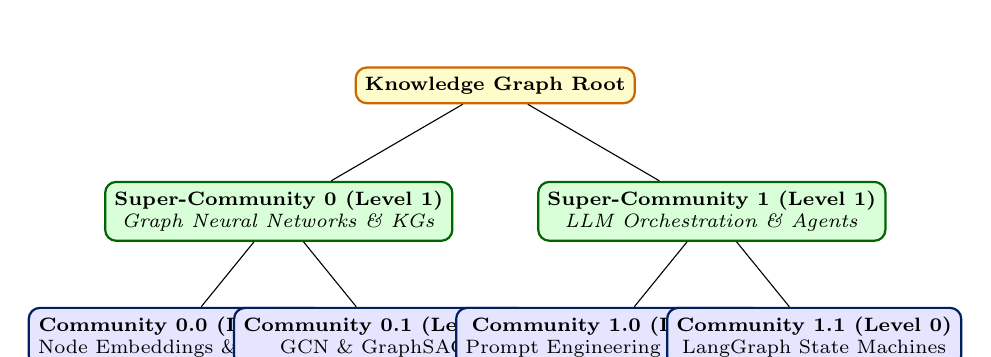
\begin{tikzpicture}[
    level 1/.style={sibling distance=5.5cm, level distance=1.6cm},
    level 2/.style={sibling distance=2.6cm, level distance=1.6cm},
    every node/.style={rectangle, draw=navyblue, fill=blue!10, rounded corners, font=\scriptsize, align=center, thick}
]
    \node [fill=yellow!20, draw=orange!80!black] {\textbf{Knowledge Graph Root}}
        child {
            node [fill=green!15, draw=darkgreen] {\textbf{Super-Community 0 (Level 1)}\\\textit{Graph Neural Networks \& KGs}}
            child { node {\textbf{Community 0.0 (Level 0)}\\\scriptsize Node Embeddings \& TransE} }
            child { node {\textbf{Community 0.1 (Level 0)}\\\scriptsize GCN \& GraphSAGE} }
        }
        child {
            node [fill=green!15, draw=darkgreen] {\textbf{Super-Community 1 (Level 1)}\\\textit{LLM Orchestration \& Agents}}
            child { node {\textbf{Community 1.0 (Level 0)}\\\scriptsize Prompt Engineering \& ReAct} }
            child { node {\textbf{Community 1.1 (Level 0)}\\\scriptsize LangGraph State Machines} }
        };
\end{tikzpicture}
\caption{Hierarchical Community Tree Generated by the Leiden Algorithm}
\label{fig:community_tree_en}
\end{figure}

\section{Neo4j GDS \& Python igraph Fallback Mechanism}
The service implements a dual-engine architecture:
\begin{enumerate}
    \item When Neo4j GDS is available, it executes \texttt{gds.leiden.write} in Neo4j memory.
    \item Otherwise, it exports nodes and edges to an in-memory \texttt{igraph.Graph} and computes partitions via \texttt{leidenalg}.
\end{enumerate}

\section{Parallel LLM Community Summarization}
After structural clustering, \texttt{CommunityDetectionService} extracts subgraph entities and relations for each community $C_k$, generating structured reports:

\begin{lstlisting}[language=Python,basicstyle=\ttfamily\scriptsize]
class CommunitySummaryReport(BaseModel):
    title: str = Field(description="Short descriptive title (max 10 words)")
    summary: str = Field(description="Comprehensive summary paragraph")
    findings: List[str] = Field(description="3-5 key insights")
    importance_score: float = Field(default=0.5, description="Significance [0.0, 1.0]")
\end{lstlisting}

Summaries are stored in \texttt{:Community} nodes and linked to member entities via \texttt{:BELONGS\_TO}.

% =============================================================================
\chapter{Advanced Graph Query \& Reasoning Engines}
% =============================================================================

\section{Query Engine Modes Overview}
The framework provides four specialized query engines:
\begin{itemize}
    \item \textbf{Local Search (\texttt{local}):} Direct entity neighborhood and chunk reranking.
    \item \textbf{Global Search (\texttt{global}):} Map-Reduce over hierarchical community summaries.
    \item \textbf{Cypher Workflow (\texttt{graph}):} Self-correcting Cypher query generation via LangGraph.
    \item \textbf{ARK Exploration (\texttt{ark}):} Adaptive multi-agent trajectory exploration.
\end{itemize}

\section{Local Search Engine}
Local search operates in 3 stages:
\begin{enumerate}
    \item \textbf{Seed Retrieval:} Finding top-$K$ seed entities using \texttt{entity\_embeddings}.
    \item \textbf{Neighborhood Expansion:} Traversing 1-hop and 2-hop edges to retrieve adjacent entities.
    \item \textbf{Synthesis:} Assembling graph triples and source chunks into the LLM synthesis context.
\end{enumerate}

\section{Global Search Engine (Map-Reduce)}
For holistic document queries, \texttt{GlobalSearchService} executes parallel Map-Reduce:
\begin{enumerate}
    \item \textbf{Filter Phase:} Vector search over \texttt{:Community} nodes at level $l$ selects top-$M$ communities.
    \item \textbf{Map Phase:} Parallel LLM execution generates partial answers $A_k^{\text{map}}$:
    \begin{equation}
        A_k^{\text{map}} = \text{LLM}_{\text{map}}(q, \text{CommunitySummary}_k, \text{Findings}_k)
    \end{equation}
    \item \textbf{Reduce Phase:} Valid partial answers are synthesized into a global answer:
    \begin{equation}
        A_{\text{final}} = \text{LLM}_{\text{reduce}}\left(q, \bigcup_{k=1}^M A_k^{\text{map}}\right)
    \end{equation}
\end{enumerate}

\section{LangGraph Cypher Query Self-Correction State Machine}
To handle complex relational queries, \texttt{workflow/graph.py} implements a LangGraph state graph.

\begin{figure}[h!]
\centering
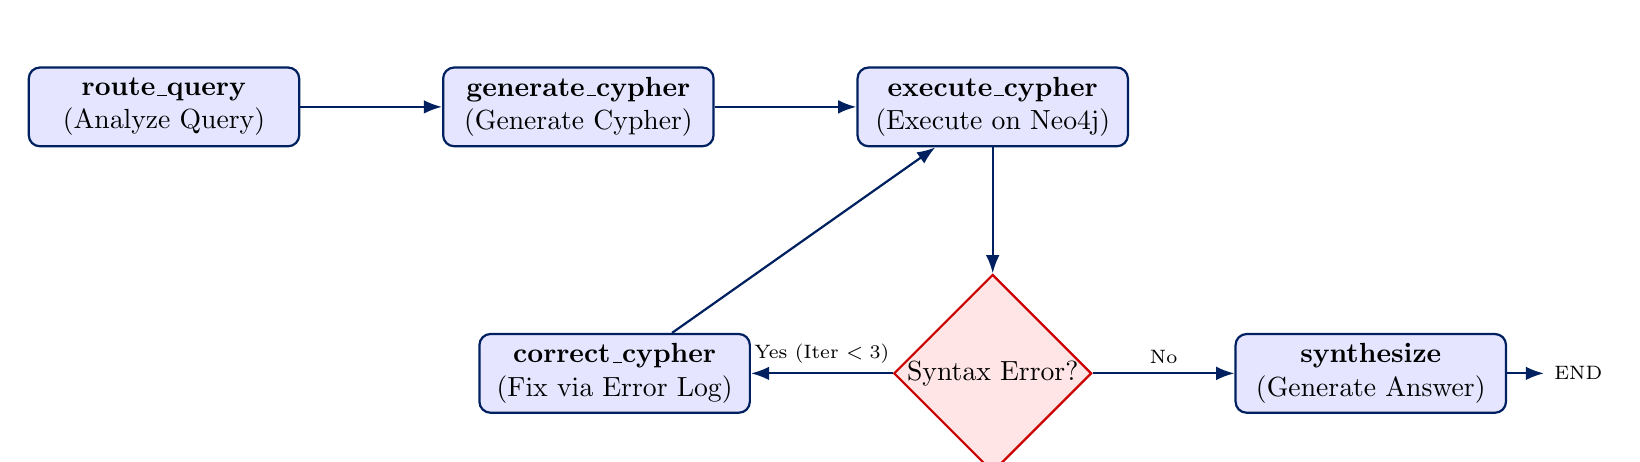
\begin{tikzpicture}[
    node distance=1.6cm and 1.8cm,
    state/.style={rectangle, draw=navyblue, fill=blue!10, thick, text width=3.2cm, align=center, minimum height=1cm, rounded corners},
    decision/.style={diamond, draw=red!80!black, fill=red!10, thick, text width=2.2cm, align=center, inner sep=0pt},
    line/.style={draw=navyblue, -Latex, thick}
]
    \node [state] (route) {\textbf{route\_query}\\(Analyze Query)};
    \node [state, right=of route] (gen) {\textbf{generate\_cypher}\\(Generate Cypher)};
    \node [state, right=of gen] (exec) {\textbf{execute\_cypher}\\(Execute on Neo4j)};
    \node [decision, below=of exec] (check) {Syntax Error?};
    \node [state, left=of check] (fix) {\textbf{correct\_cypher}\\(Fix via Error Log)};
    \node [state, right=of check] (synth) {\textbf{synthesize}\\(Generate Answer)};

    \path [line] (route) -- (gen);
    \path [line] (gen) -- (exec);
    \path [line] (exec) -- (check);
    \path [line] (check) -- node[above] {\scriptsize Yes (Iter $< 3$)} (fix);
    \path [line] (fix) -- (exec);
    \path [line] (check) -- node[above] {\scriptsize No} (synth);
    \path [line] (synth) -- ++(2.2,0) node[right]{\scriptsize END};
\end{tikzpicture}
\caption{LangGraph State Machine for Self-Correcting Cypher Queries}
\label{fig:cypher_state_graph_en}
\end{figure}

The state is tracked via \texttt{GraphRAGState}:
\begin{lstlisting}[language=Python,basicstyle=\ttfamily\scriptsize]
class GraphRAGState(TypedDict):
    query: str
    routing: str           # "vector", "graph", "hybrid"
    cypher_query: str
    cypher_records: List[Dict[str, Any]]
    graph_context: str
    response: str
    error: str
    iteration: int
    schema: str
\end{lstlisting}

If execution fails, \texttt{correct\_cypher} sends the database schema, failing Cypher statement, and Neo4j error log to the LLM for correction (capped at 3 iterations).

\section{ARK Multi-Agent Adaptive Exploration Engine}
The \textbf{ARK} engine executes parallel stochastic exploration across $N=3$ agents ($T=0.7$, $t_{\text{max}}=30$).

\subsection{Agent Toolset}
Each agent operates with 4 action tools:
\begin{enumerate}
    \item \texttt{global\_search}: Seed entity lookup via fulltext/vector index.
    \item \texttt{neighborhood\_exploration}: 1-hop neighbor exploration from a given entity.
    \item \texttt{add\_to\_answer}: Selecting a node with explicit reasoning.
    \item \texttt{finish}: Terminating exploration once sufficient context is acquired.
\end{enumerate}

\subsection{Voting Rank Fusion (VRF)}
Candidate nodes selected across all agent trajectories $\mathcal{S}_1, \dots, \mathcal{S}_N$ are aggregated via Voting Rank Fusion:
\begin{equation}
    \text{Score}(u) = \sum_{a=1}^N \mathbb{I}(u \in \mathcal{S}_a) \cdot \left[ 1.0 + \frac{1.0}{1.0 + \text{order}_a(u)} \right]
\end{equation}
The top-$K$ scoring nodes are formatted into the final LLM context.

% =============================================================================
\chapter{System Architecture \& Monorepo Design}
% =============================================================================

\section{Monorepo UV Workspace Architecture}
The codebase is structured as a modular monorepo managed via \textbf{uv workspaces} (\texttt{RAG\_package/pyproject.toml}):

\begin{figure}[h!]
\centering
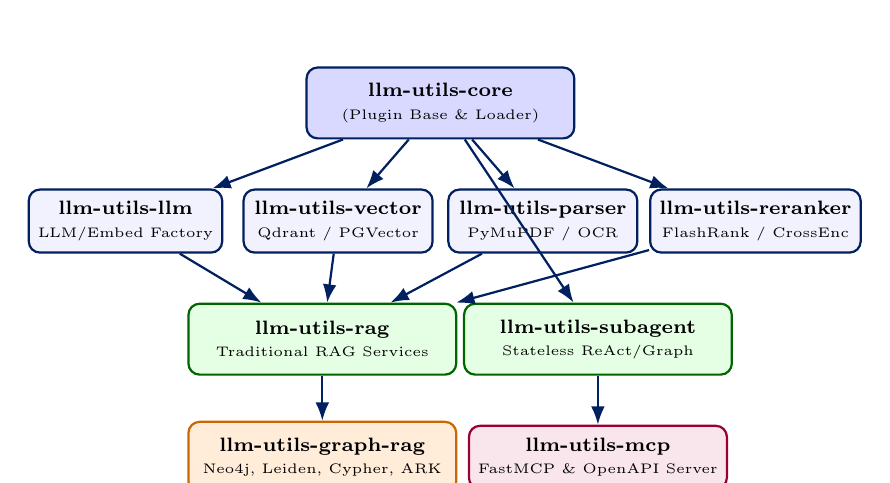
\begin{tikzpicture}[
    every node/.style={font=\scriptsize, align=center, thick},
    pkgCore/.style={rectangle, draw=navyblue, fill=blue!15, rounded corners, minimum height=0.9cm, minimum width=3.4cm},
    pkgBase/.style={rectangle, draw=navyblue, fill=blue!5, rounded corners, minimum height=0.8cm, minimum width=2.4cm},
    pkgApp/.style={rectangle, draw=darkgreen, fill=green!10, rounded corners, minimum height=0.9cm, minimum width=3.4cm},
    pkgExt/.style={rectangle, draw=purple!80!black, fill=purple!10, rounded corners, minimum height=0.8cm, minimum width=3.2cm},
    depLine/.style={draw=navyblue, -Latex, thick}
]
    \node [pkgCore] (core) at (4, 4.5) {\textbf{llm-utils-core}\\\tiny (Plugin Base \& Loader)};

    \node [pkgBase] (llm) at (0, 3) {\textbf{llm-utils-llm}\\\tiny LLM/Embed Factory};
    \node [pkgBase] (vec) at (2.7, 3) {\textbf{llm-utils-vector}\\\tiny Qdrant / PGVector};
    \node [pkgBase] (parse) at (5.3, 3) {\textbf{llm-utils-parser}\\\tiny PyMuPDF / OCR};
    \node [pkgBase] (rerank) at (8, 3) {\textbf{llm-utils-reranker}\\\tiny FlashRank / CrossEnc};

    \node [pkgApp] (rag) at (2.5, 1.5) {\textbf{llm-utils-rag}\\\tiny Traditional RAG Services};
    \node [pkgApp] (sub) at (6, 1.5) {\textbf{llm-utils-subagent}\\\tiny Stateless ReAct/Graph};

    \node [pkgCore, fill=orange!15, draw=orange!80!black] (graphrag) at (2.5, 0) {\textbf{llm-utils-graph-rag}\\\tiny Neo4j, Leiden, Cypher, ARK};
    \node [pkgExt] (mcp) at (6, 0) {\textbf{llm-utils-mcp}\\\tiny FastMCP \& OpenAPI Server};

    \path [depLine] (core) -- (llm);
    \path [depLine] (core) -- (vec);
    \path [depLine] (core) -- (parse);
    \path [depLine] (core) -- (rerank);

    \path [depLine] (llm) -- (rag);
    \path [depLine] (vec) -- (rag);
    \path [depLine] (parse) -- (rag);
    \path [depLine] (rerank) -- (rag);

    \path [depLine] (rag) -- (graphrag);
    \path [depLine] (core) -- (sub);
    \path [depLine] (sub) -- (mcp);
\end{tikzpicture}
\caption{Workspace Package Dependency Architecture in uv Monorepo}
\label{fig:monorepo_architecture_en}
\end{figure}

\section{Package Overview}
\begin{enumerate}[leftmargin=*]
    \item \textbf{\texttt{llm-utils-core}:} Plugin interface base classes and dynamic loader logic.
    \item \textbf{\texttt{llm-utils-llm}:} Unified factory supporting OpenAI and Anthropic Claude APIs.
    \item \textbf{\texttt{llm-utils-vector}:} Qdrant and PostgreSQL \texttt{pgvector} vector store providers.
    \item \textbf{\texttt{llm-utils-parser}:} Document parsers (PyMuPDF, Docling, Office) and OCR integration.
    \item \textbf{\texttt{llm-utils-reranker}:} Second-stage rerankers (FlashRank, CrossEncoder).
    \item \textbf{\texttt{llm-utils-graph-rag}:} Neo4j Graph RAG, Leiden community detection, and ARK engine.
    \item \textbf{\texttt{llm-utils-mcp}:} FastMCP server exposing tools over RESTful OpenAPI on port \texttt{8001}.
\end{enumerate}

\section{Backend Services \& Lazy Singleton Registry}
The FastAPI backend (\texttt{BE/}) manages services via a thread-safe lazy singleton registry (\texttt{GraphRAGServiceRegistry} in \texttt{registry.py}):

\begin{lstlisting}[language=Python,basicstyle=\ttfamily\scriptsize]
class GraphRAGServiceRegistry:
    _instance: Optional["GraphRAGServiceRegistry"] = None
    _lock = threading.Lock()

    def __new__(cls, config: Optional[AppConfig] = None):
        with cls._lock:
            if cls._instance is None:
                cls._instance = super().__new__(cls)
                cls._instance._initialized = False
            return cls._instance
\end{lstlisting}

This pattern guarantees thread-safe, single-instance initialization of Neo4j connection pools and embedding models across all concurrent requests.

% =============================================================================
\chapter{Discussion, Technical Challenges \& Future Work}
% =============================================================================

\section{Architectural Discussion}
Combining symbolic Property Knowledge Graphs with sub-symbolic vector embeddings provides:
\begin{itemize}[leftmargin=*]
    \item \textbf{Explainability:} Every fact is linked to labeled graph edges with clear document provenance (\texttt{source\_documents}).
    \item \textbf{Query Flexibility:} Four specialized query modes seamlessly address both pinpoint factual queries and corpus-wide macro summaries.
\end{itemize}

\section{Technical Challenges}
\begin{enumerate}[leftmargin=*]
    \item \textbf{Indexing Computation Overhead:} Entity/relation extraction and Leiden community summarization incur significant LLM token costs during initial indexing.
    \item \textbf{Dynamic Incremental Graph Updates:} Re-clustering the entire graph when adding/deleting documents is computationally expensive, necessitating incremental Leiden partitioning algorithms.
\end{enumerate}

\section{Future Directions}
\begin{enumerate}[leftmargin=*]
    \item \textbf{Multimodal Knowledge Graphs:} Extracting tables, architectural diagrams, and mathematical formulas directly into graph nodes.
    \item \textbf{Reinforcement Learning for Graph Traversal:} Training RL agents to optimize navigation policies across massive knowledge graphs.
\end{enumerate}

% =============================================================================
\chapter{Conclusion \& Task Division}
% =============================================================================

\section{Conclusion}
This project successfully designed and implemented \textbf{HLG LLM Utils}, a robust, production-grade Graph RAG framework. By integrating Neo4j Property Knowledge Graphs, Hierarchical Leiden Community Detection, LangGraph Cypher Query Self-Correction, and ARK multi-agent traversal, the framework resolves the fundamental limitations of Naive RAG and provides a solid foundation for enterprise-scale knowledge representation and reasoning.

\section{Student Contribution Matrix}

\begin{table}[h!]
\centering
\caption{Task Division Matrix Between Group Members}
\label{tab:task_division_en}
\small
\begin{tabularx}{\textwidth}{>{\raggedright\arraybackslash}p{3.8cm} >{\centering\arraybackslash}p{2.2cm} X >{\centering\arraybackslash}p{1.8cm}}
\toprule
\textbf{Student Name} & \textbf{ID} & \textbf{Specific Contributions \& Key Responsibilities} & \textbf{Contribution} \\
\midrule
\textbf{Nguyen Hoai Nam} & 25C01014 &
\begin{itemize}[leftmargin=*,noitemsep,topsep=0pt,partopsep=0pt,parsep=0pt]
\item Designed Monorepo \texttt{uv workspace} architecture (\texttt{llm-utils-core}, \texttt{llm-utils-graph-rag}).
\item Implemented Neo4j Graph Store and Hierarchical Leiden Community Detection (\texttt{community.py}).
\item Built Map-Reduce Global Search engine (\texttt{global\_search.py}).
\item Authored academic LaTeX report documentation.
\end{itemize} & 50\% \\[0.2cm]
\midrule
\textbf{Pham Cung Le Nhan Vu} & 25C01049 &
\begin{itemize}[leftmargin=*,noitemsep,topsep=0pt,partopsep=0pt,parsep=0pt]
\item Built LangGraph Cypher Query Self-Correction state graph (\texttt{workflow/graph.py}).
\item Implemented ARK Autonomous Multi-Agent Traversal framework (\texttt{ark\_agent.py}, \texttt{ark\_retriever.py}).
\item Engineered FastAPI backend and Qdrant / PGVector integrations.
\item Optimized retrieval performance and finalized system integration.
\end{itemize} & 50\% \\
\bottomrule
\end{tabularx}
\end{table}

% -----------------------------------------------------------------------------
% REFERENCES
% -----------------------------------------------------------------------------
\newpage
\addcontentsline{toc}{chapter}{References}
\bibliographystyle{plain}
\bibliography{references}

\end{document}
